\documentclass{ieeeaccess}
\usepackage[UTF8]{ctex} 
\usepackage{cite}
\usepackage{amsmath,amssymb,amsfonts}

\usepackage{booktabs}
\usepackage{array}
\usepackage{multirow}
\usepackage{longtable}
\usepackage{rotating}
\usepackage[utf8]{inputenc} % allow utf-8 input
\usepackage[T1]{fontenc}    % use 8-bit T1 fonts


\usepackage{algorithmic}
\usepackage{subfigure}
\usepackage{graphicx}
\usepackage{textcomp}
\def\BibTeX{{\rm B\kern-.05em{\sc i\kern-.025em b}\kern-.08em
    T\kern-.1667em\lower.7ex\hbox{E}\kern-.125emX}}
\begin{document}
\history{Date of publication xxxx 00, 0000, date of current version xxxx 00, 0000.}
\doi{10.1109/ACCESS.2017.DOI}

\title{Preparation of Papers for IEEE ACCESS}
\author{\uppercase{Hao Li}\authorrefmark{1}, \IEEEmembership{Member, IEEE},
\uppercase{Second B. Author\authorrefmark{2}, and Third C. Author,
Jr}.\authorrefmark{3},
\IEEEmembership{Member, IEEE}}
\address[1]{Beijing University of chemical and technology, Beijing, 10029 China (e-mail: 2018040206@mail.buct.edu.cn)}
\address[2]{Department of Physics, Colorado State University, Fort Collins, 
CO 80523 USA (e-mail: author@lamar.colostate.edu)}
\address[3]{Electrical Engineering Department, University of Colorado, Boulder, CO 
80309 USA}
\tfootnote{This paragraph of the first footnote will contain support 
information, including sponsor and financial support acknowledgment. For 
example, ``This work was supported in part by the U.S. Department of 
Commerce under Grant BS123456.''}

\markboth
{Author \headeretal: Preparation of Papers for IEEE TRANSACTIONS and JOURNALS}
{Author \headeretal: Preparation of Papers for IEEE TRANSACTIONS and JOURNALS}

\corresp{Corresponding author: First A. Author (e-mail: author@ boulder.nist.gov).}

\begin{abstract}
  In recently years, deep learning-based models brought about performance breakthrough  in medical image community. For image segmentation, registration and reconstruction tasks, deep models consistently outperforms traditional methods. Specifically, the U-Net model proposed by Olaf Ronneberger \emph{et al.}\cite{RonnebergerFB15} and some variants are becoming the de facto standard model and widely used in various medical image tasks. Despite great success, it is still a challenge task to accurately segment and identify the location and sizes of rectal tumors. Another challenge is the amorphous or irregularly shaped boundaries of object. In this study, we propose a novel U-Net architecture to address the aforementioned issues regarding segment performance and shape identification. our model mainly includes two improvements on U-Net. Firstly, we re-design the skip pathways with spatial and channel attentions which reduce the semantic gap between the feature maps of encoder and decoder sub-networks. Secondly, a novel loss function was proposed to emphasize the segmentation accuracy on tumor boundaries and encourages shape feature preservation. We have evaluated the ASU-Net in comparison with U-Net and some variants on multiple medical image segmentation tasks: liver segmentation in abdominal CT scans, nodule segmentation in the low-dose CT scans. Based on the experimental results, it was identified that the proposed method performed a significant role in improving accuracy and shape preservation.
  \end{abstract}

\begin{keywords}
U-Net, Biomedical image segmentation, Attention
\end{keywords}

\titlepgskip=-15pt

\maketitle

  
  % 这篇文章的中心思想就是研究Attention和损失函数来改进U-Net网络
  \section{Introduction}
  % 深度学习在医疗领域里获得了成功的应用.
  Medical images of different modality such as tomography (CT), positron emission tomography (PET), X-ray, Ultrasonic, and singlephoton emission computed tomography (SPECT) play an increasingly important role for clinician to analyse and diagnosis of diseases. For example, Diabetic Retinopathy (DR), which  is a universal retinal disease caused by elevated blood sugar, accompanied by retinal vascular swelling. Early detection and treatment are the keys to determine the degree and severity of vitreoretinal traction. Ultrasound is a valuable diagnostic tool for this disease, which can evaluate the state of the retina in vitreous hemorrhage or vitreous opacity.
  %Automated medical image analysis has been extensively studied in the medical imaging community due to the fact that manual labelling of large amounts of medical images is a tedious and error-prone task.
  
  In general, medical image analysis including image segmentation, object detection and tracking tasks can be categorized into two classes. (1) manual and semi-automatic segmentation, (2) automatic segmentation.  The traditional manual analysis requires physicians, radiologists, or experts with advanced technical knowledge to carry out the tasks. Furthermore, the segmentation quality relies heavily on the judgement of experts. The segmentation and diagnosis process is rather time-consuming and error-prone. In the past few decades, researchers have proposed a great number of methods for automatic segmentation, detection and tracking in Medical Image Community. Early methods were based on traditional pattern recognition techniques like statistical modeling and edge detection filters. For example, Bankhead et al\cite{PeterNGT12} proposed a wavelet-based method to enhance the detection of vessel foreground and background. Later, machine learning approaches using hand-crafted features based on the modality and type of segmentation task were developed. For instance, Lupascu \emph{et al.} \cite{LupascuTT10} designed 41-$D$ feature vectors for every pixel to train the AdaBoost classifier to classify each pixel in the retinal images. 
  %However, the manual annotating of retinal vessels by ophthalmologists is a slow and laborintensive task, so researchers have devoted themselves to proposing automatic retinal vessel segmentation methods
  
  With the advent of deep learning, convolutional neural networks (CNNs) have been showing promising results over the conventional methods in medical image tasks like image segmentation, registration and tracking and so on. Medical image segmentation is an important task of artificial intelligence assisted medical technology. The automatic segmentation of medical image not only help clinician identify the candidate regions, but also give helpful diagnosis suggestions. During the past decade, many effective models have been developed by researchers. The classic model is fully convolutional network (FCN) proposed by Jonathan Long et al\cite{LongSD15}. Fully convolutional networks (FCN) take advantage of fully convolutional layers to train a segmentation model in an end-to-end way by replacing fully connected layers in CNN with convolutional layers. Despite outstanding performances, FCN suffers from conceptual limitations in complex segmentation tasks, e.g. when dealing with local visual ambiguities and low contrast between organs. Since then,  several variants have been developed for medical image segmentation tasks like SegNet, U-Net and so on. What is worth noting is that most architectures developed for semantic segmentation in both computer vision and medical medical images are encoder-decoder type convolutional networks. SegNet was the first encoder-decoder type convolution networks. A major breakthrough in medical image segmentation was U-Net architecture proposed by Olaf Ronneberger\cite{RonnebergerFB15} which has recently become backbone of almost all the leading models. Subsequently, a variety of network architectures based on U-Net are proposed to enhance the segmentation performance. Several main extensions includes UNet++, Attention Gate UNet, UNet-Transformer, Double U-Net, TVUNet and so on. In addition, extensions like 3D U-Net and V-Net are also proposed for volumetric segmentation in 3D medical scans. It is worth noting that all the above extensions of U-Net used the same encoder-decoder architecture and their contributions were either in encoder and decoder, using different convolutional layer or in skip connections, using different concatenation to combine the features in appropriate level. 
  %Although deep learning demonstrates increasing applications, the lack of annotated medical image data results in difficulty in successfully deploying CNNs in the clinics.
  
  % 存在的问题
  Despite the success of U-Net and its variants,  there are some disadvantages of above networks. In general, U-Net and its variants are good at segmenting large structure, they fail when the segment objects are small or have noisy boundaries which can be seen in Fig \ref{fig:segment_small_structures}. From the figure above, the U-Net architecture lacks focus in extracting features for segmentation of small structures. 
  \begin{figure*}[htbp]
  \small
  \centering
  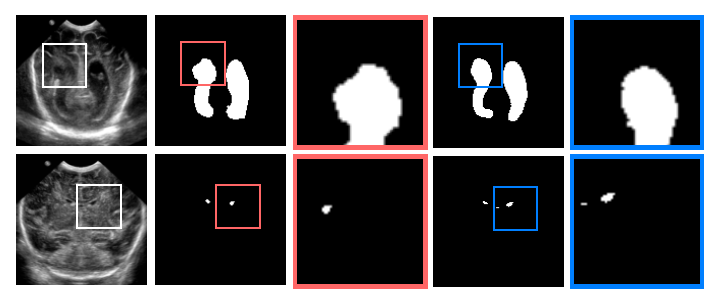
\includegraphics[width=0.8\textwidth]{figure/segment_small_structures.png}
  \label{fig:segment_small_structures}
  \caption{small structure segmentation}
  \end{figure*}
  
  In addition, UNet network also faces the challenge to segment objects with enough good accuracy for retina segmentation due to 
  shape variability and unclear boundaries of segmenting objects. In encoder part of network, feature extraction process is often performed by CNN networks which are are highly influenced by dense pixel values which are not robust features compared to shapes of objects. From the perspective of evaluation,  most segmentation evaluation metrics to quantify segmentation performance, such as accuracy, spedificity, and jaccard similarity, do not directly reflect how well a object boundary is delineated which hinders to segment object with clear boundaries. Last but not least,  UNet architecture family also shared the disadvantage by deep neural network is a lack of interpretability. 
  
  % 本文的解决方法
  To address the issues illustrated above in medical image segmentation, in this paper, we proposed a new UNet variant named SA-UNet. The proposed model is inspired by growing interest on integrating attention mechanisms and shape-aware feature preservation in image segmentation networks for natural scenes. Attention mechanism has been shown to be a powerful technique in deep learning models and has been widely used in various tasks in natural language processing to capture keywords for context. Unlike the previous approaches, SA-UNet re-design the skip-connection to fuse several different attention mechanisms including spatial attention, channel-wise attention and self-attention. Spatial attention focus on some special region which contains the objects to be segmented; channel-wise attention vector are employed in the lower resolution to extract feature in some channel. self-attention effectively captures the long-range dependencies between visual features. Despite the growing interest on integrating attention mechanisms in medical image segmentation scenes, the adoption of several attention mechanisms in medical images remains scarce, being limited to simple attention models. Furthermore, we also consider shape-feature perservation in feature extraction procedure in imporved implemenation in the loss function.  The shapes of objects should be learned to allow generalizability and robustness of the model which goes hand-in-hand with transparency which also increases the interpretability in a clinical setting. There are several advantages of our proposed architectures for segmentation task. Fristly, The new model augmented with multi-attention improves the performance in a variety of  segmentation tasks. Secondly new loss function contributes to the shape preservation of objects to be segmented. The experimental results show superior performance on segmentation tasks compared to equivalent models including U-Net and serveral variants. 
  
  % 本文主要贡献
  The contributions of this work can be summarized as follows:
  \begin{enumerate}
  \item We propose a novel multi-attention module that can be utilised in CNN based standard image analysis models for classification, segmentation and tracking application and so on.
  \item We redesign the skip-connection to fuse different attention mechanisms and proposed the SAU-Net architecture for medical image segmentation task. 
  \item The architecture use new loss function for shape preservation for medical image analysis, in particular, in the context of image classification and segmentation.
  \end{enumerate}
  
  % Paper structure.
  The remainder of this paper is organized as follows.. In Section \ref{sec:related}, we introduce background knowledge, including U-Net architecture family, existing attention mechanism and shape-aware related work in machine learning fields. Section \ref{sec:method} introduce the proposed method, including network architecture and attention modules and new loss function to preserve the shape feature. in Section \ref{sec:experiment}, we give some experiment and present the results in detail and section \ref{sec:conc} conclude the paper.
  
  \section{Related work}\label{sec:related}
  In this section, we review several lines of research related to our work in the following felds.
  % U-Net Variants
  \paragraph{U-Net and variants} In medical image segmentation, Fully Convolution Networks (FCN) have been widely used for semantic segmentation and contextual aggregation. In 2015, Olaf Ronneberger \emph{et al.} proposed a U-shape architecture that employs contracting and expanding paths together with skip connections, which combines both low-and high-level features for image segmentation\cite{RonnebergerFB15}. With UNet as a backbone, researchers proproosed improved variants for volumetric segmentation in 3D medical scans, such as 3DUNet\cite{CicekALBR16} and V-Net\cite{MilletariNA16}. Zongwei Zhou \emph{et al.} proposed UNet++, a new segmentation architecture based on nested and dense skip connections \cite{ZhouRTL18}. The architecture can more effectively capture fine-grained details of the foreground objects when high-resolution feature maps are gradually fusioned from encoder and decoder network. Wen Liu \emph{et al.} presented an enhanced nested U-Net architecture named MDAN-UNet for segmentation of OCT images\cite{LiuSJ20}. The approach designed a UNet++ alike network and redesigns the skip pathways, multi-scale input, multi-scale side output and accurately segment pixels of OCT images. Nabil Ibtehaz \emph{et al.} propose some modifications to improve upon the already state-of-the-art U-Net model\cite{IbtehazR20}. They replaces the convolutional layers with Inception-like blocks should facilitate the U-Net architecture to reconcile the features learnt from the image at different scales. They also introduced residual connections to them as they make the learning easier. Kevin Trebing et al propose SmaAt-UNet, an efficient convolutional neural networks based on the well known UNet architecture equipped with attention modules and depthwise-separable convolutions\cite{TrebinM20}.    
  
  % Attention
  \paragraph{Attention}
  In recent years, attention has been a fairly popular concept and useful mechanism in deep learning community. Attention mechanism has been shown to be a powerful technique in deep learning models and has been widely used in various tasks in natural language processing to capture keywords for context. Some attention mechanisms and models, such as transformer and SNAIL are nearly becoming the de facto standard components of deep networks. In fact, the idea of attention is intuitive and simple, for an image, our visual system always focuses on some object of interest in the image, rather than focusing on the whole image. Inspired by the successful application of attention mechanism, Sahar Yousefi et al proposed Attention U-Net with Dilated Dense Attention for automatically segmenting the esophageal tumor\cite{YousefiSELMZDS20}. The model introduced dilated dense spatial attention and channel attention blocks which are composed of dilated dense block (DDB) and a spatial attention gate and a channel attention gate. Jo Schlempera \emph{et al.} introduce attention mechanism named Attention Gate (AG) which can be flexibly incorporated in existing CNN segmentation and classification architectures\cite{OktaySFLHMMMHKGR18}. Attention Gate mechanism also provides fine-scale attention maps that can be visualized, with minimal computational overhead. The experiments on 3D-CT abdominal image and 2D fetal ultrasound show increased sensitivity while not sacrificing specificity. Yancheng Lan \emph{et al.} designed an novel encoder-decoder network using mixed-attention mechanism (MARU) to reconstruct the ultrasound image\cite{LanZ20}. During the encoding phase, a lightweight mixed-attention block is designed to effectively enhance the image features and suppress some speckle noise. Haijun Gao et al proposed DPU-Net model further modified the U-Net structure which has only one path to two contracting paths\cite{GaoZPZ20}. DPU-Net has the function of covariance self-attention which is embedded into the up-sampling and bottom block sub-modules. The main advantage of DPU-Net not only integrates multi-scale semantic information, but the decoder can obtain sufficient fine-grained and coarse-grained semantic information at multiple scales. Mehrdad Noori \emph{et al.} proposed an attention-guided extension of UNet network for Brain Tumor Segmentation in which two techniques are employed\cite{NooriBM20}. Firstly, an attention mechanism is adopted after concatenation of low-level and high-level features. Secondly, multi-views are fused from 3D contextual information of input images to enrich feature maps despite using a 2D model. Chen Li \emph{et al.} incorporated the Attention Gate mechanism into nested UNet architecture and proposed the attention UNET++. The model redesigned dense skip connection and increased the weight of the target region while inhibiting the background region\cite{LiTCLGJW20}. Changlu Guo \emph{et al.} presented Channel Attention Residual U-Net(CAR-UNet) model which considers the relationship between the feature channels to strengthen the discriminative capability\cite{GauSYZ20}. 
  %The self-attention mechanism, also known as internal attention mechanism, calculates the corresponding semantic information through modeling the relationship between different positions in a single sequence, and then directly models the remote information interaction between semantics.
  %In particular, given a sequence of text and a current word, a task is to extract a next word in a sentence generation or translation. The idea of attention mechanisms is to generate a context vector which assigns weights on the input sequence.
  
  % Shape
  \paragraph{Shape} The existing deep learning models for medical image segmentation are usually based on traditional loss functions that only regard objects at pixel level. Obviously, the medical images that suffer from low-quality and low signal-to-noise ratio without any shape constraint remains problematic even for deep models. Some works has been shown that incorporation of shape prior information significantly improves the performance of the segmentation algorithms, incorporation of such prior knowledge is a tricky practical problem. In general, incorporation of shape prior information can be devided into three main categories: 1) Conditional or Markov Field models that establish connections between different pixel regions; 2) Active/Statistical Shape Models that learn a special representation for valid shapes; 3) Active Contour Models or snakes that use deformable splines for shape detection;
  
  These models are either applied as pre-processing steps to create initial segmentations, post-processing steps to refine the neural network segmentations, or used in multi-step models consisting of various models along a specific pipeline.
  
  %do not incorporate any form of shape knowledge. 
  %Incorporating prior knowledge into traditional image segmentation algorithms has proven useful for obtaining more accurate and plausible results.
  %Though it has been shown that incorporation of shape prior information significantly improves the performance of the segmentation algorithms  
  
  % 本文提出的方法详细阐述
  \section{Proposed Method}\label{sec:method}
  Our novel architecture is inspired from the attention UNet, which uses attention to give importance to a certain region out
  of the entire image.
  
  %这里描述提出的方法,先描述模型整理,然后再描述模型的部分和细节内容。有些内容用数学语言来进行阐述。
  
  Different from the original UNet architecture we have used attention gates which take the features from the encoder and the output of the pyramid pool as input and produced out-put is further concatenated with the up-sampled output of the previous pyramid-pool layer and mapped to the next subsequent layer. This network can map local features with their global counterparts with improved accuracy and emphasize on discriminative image regions by focusing on relevant local features only.
  
  \subsection{Architecture}
  U-Net\cite{unet} architecture has shown remarkable performance and potential in medical image segmentation tasks. 
  However, deep neural network would occur the model degradation problem. To overcome the above problem, ResU-Net replaces the typical convolutional sequence module with ResNet-34 \cite{HeZRS16} as feature encoder.
  
  In our purposed method, we use the pretrained ResU-Net\cite{ResUNet} as our backbone approach, which is shown in Figure \ref{fig:overview}.
  
  \begin{figure*}[htbp]
  \small
  \centering
  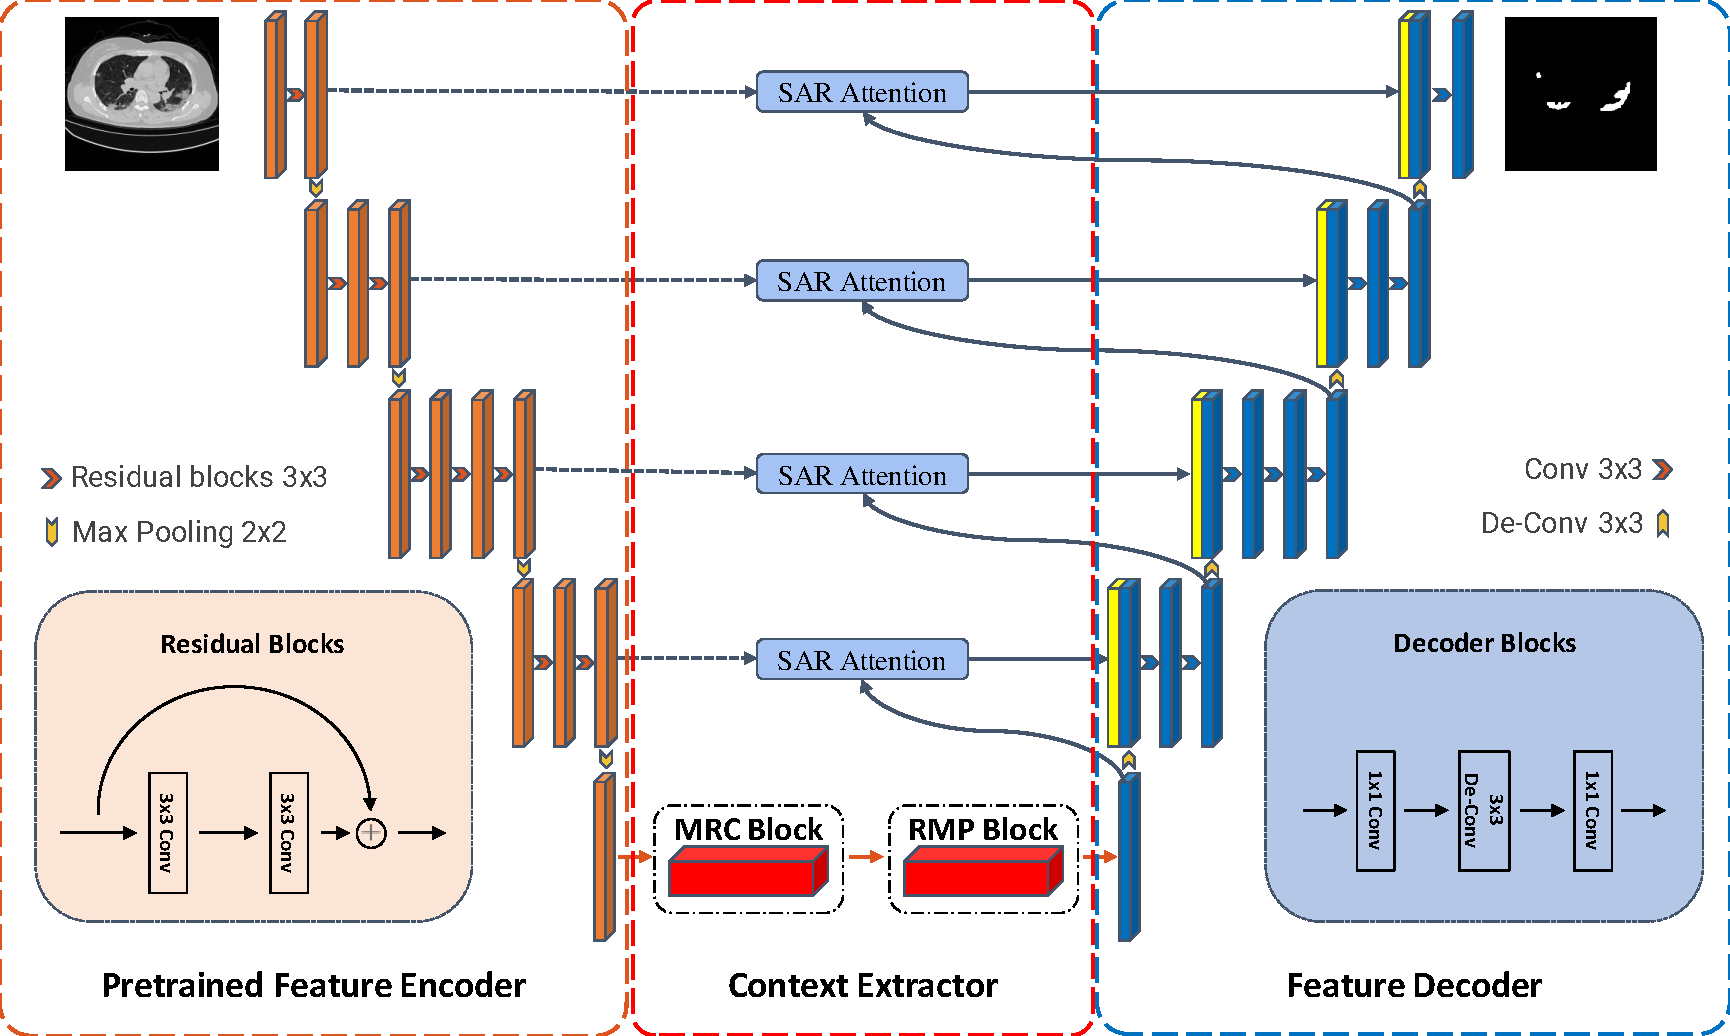
\includegraphics[width=1\textwidth]{figure/overview.pdf}
  \label{fig:overview}
  \caption{EA-UNet Architecture}
  \end{figure*}
  
  \subsection{Multi residual convolutional blocks}
  It has been proved that high-level feature maps are significant for semantic segmentation tasks. In calssical U-Net like architecture, a sequence of two \(3\times 3\) convolutional layers are used to extract high-level semantic feature maps,
  As Christian \emph{et al.} mentioned in inception\cite{SzegedyVISW16},  this series of two $3 \times 3$ convolutional operation actually resembles a $5 \times 5$ convolutional operation, which is not conductive to our network 
  learning its features on different scales.
  
  Hence following the approach idea, the simplest way to augment U-Net's performance with multi-resolutional analysis is to incorporate \(3\times 3, 5\times 5, 7\times 7\) convolution operations, as what Inception\cite{SzegedyVISW16} did.
  Gu \emph{et al.} proposed CE-Net\cite{cenet}, it demonstrated the DAC block(dense atrous convolution module) to combine shortcut connection with inception-series structures.
  It did gain the performance. Nevertheless, the memory requirements of this method are increasing extravagantly. Therefore, 
  
  \begin{figure}[htbp]
    \small
    \centering
    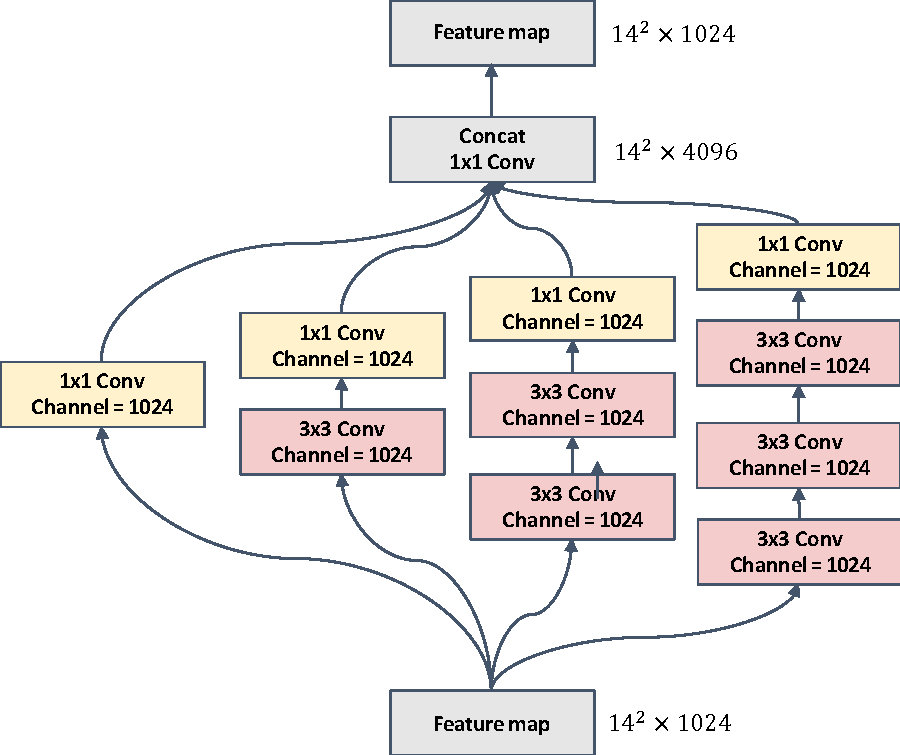
\includegraphics[width=0.35\textwidth]{figure/DAC_block.pdf}
    \label{fig:dac_block}
    \caption{DAC BLock}
  \end{figure}
  
  
  Motivated by CE-Net\cite{cenet} and MultiResUNet\cite{IbtehazR20}: instead of using three sequences of \(3\times 3\) filters in parallel, 
  we decide to use only one succession of \(3 \times 3\) lightweight convolutional blocks, the outputs of 2nd and 3rd can be approximately considered as \(5\times 5\) and \(7 \times 7\) convolution operations. Then we take the outputs from the three convolutions blocks and then concatenate
  them to extract high-level semantic feature from different resolutions. We call this arrangement  \emph{'multi residual convolutional block'}, as shown in Figure \ref{fig:mrc_block}.
  
  \begin{figure}[htbp]
    \small
    \centering
    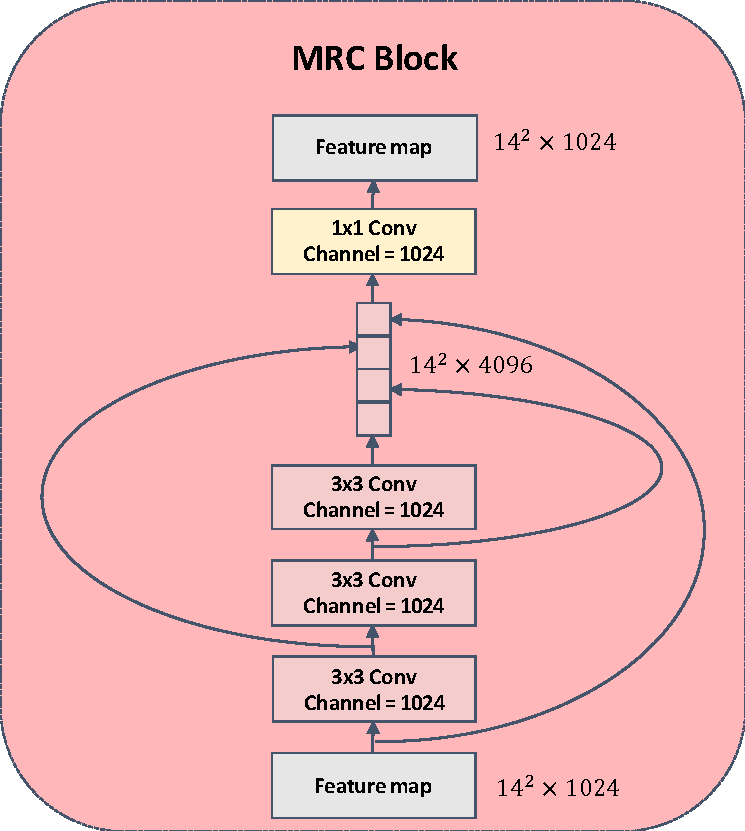
\includegraphics[width=0.35\textwidth]{figure/MRC_block.pdf}
    \label{fig:mrc_block}
    \caption{MRC BLock}
  \end{figure}
  
  通过上述对模型的修改,我们能够
  \begin{table}[htbp]
    \vspace{-2mm}
    \begin{center}\small
    \label{param-table}
    \begin{tabular}{ccccccc}
      
    \toprule
    Backbone & Components & Params & Params size \\
    \midrule
      CE-Net & SAR & 135,571,137 & 517.16 \\
      ResU-Net & SAR+ASPP    & 92,573,377 & 353.14  \\
      ResU-Net & SAR+MRC+RMP & 94,669,505 & 361.14  \\
  \bottomrule    
    \end{tabular}
    \caption{Memorize Cost Comparison With Different Methods In Bottleneck}
  \end{center}
    %\vspace{-0.35cm}
    \vspace{-4mm}
  \end{table}
  
  \subsection{Residual Multi-kernel pooling}
  The large variation of object size in medical image is a big challenge in medical image segmentation. Take COVID19 lesion for example, the lesion size may be very different for different patients.
  CE-Net proposed residual multi-kernel pooling module to encode more context information through different-size receptive fields: \(2\times 2\), \(3\times 3\), \(5\times 5\) and \(6 \times 6\). 
  After the pooling layers, we use \(1\times 1\) convolution to encode the context information and then upsample to the origianl size, which makes us easy to concatenate the origianl feature maps. 
  At this point, the dimensions of feature maps has come to \(5N\), where \(N\) represents the number of channels in origianl feature maps.
  Finally, we use \(1\times 1\) convolution to reduce the channel down to \(N\).
  \begin{figure}[htbp]
    \small
    \centering
    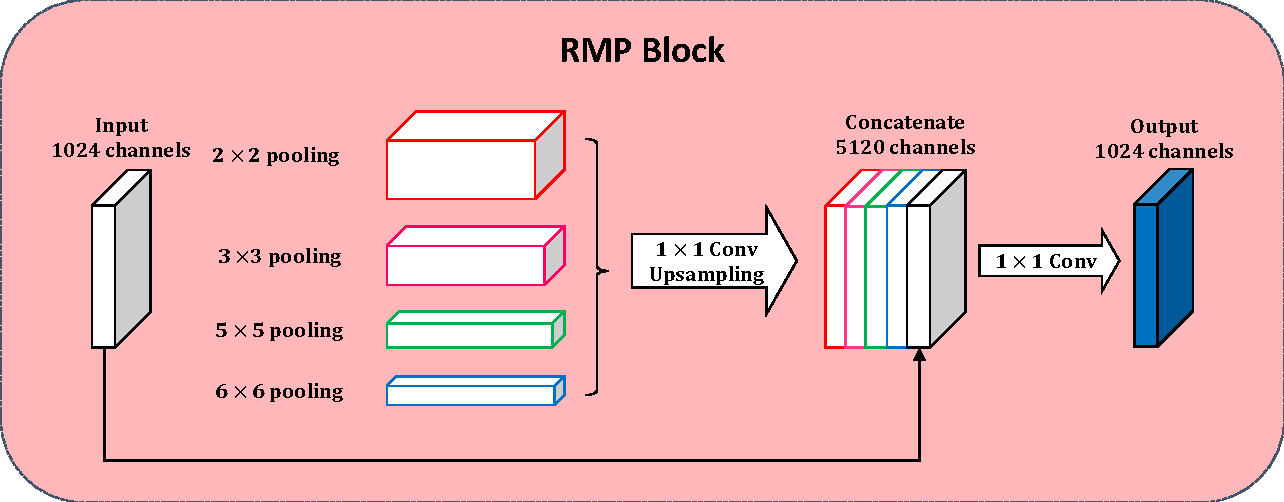
\includegraphics[width=0.49\textwidth]{figure/rmp_block.pdf}
    \label{fig:rmp_block}
    \caption{RMP BLock}
  \end{figure}
  \subsection{Attention Ensemble}
  
  There are two commonly used attention types: multiplicative (Luong \emph{et al.}, 2015) and additive attention (Bahdanau \emph{et al.}, 2014). The former is faster to compute and more memory-efficient in practice since it can be implemented as a
  matrix multiplication. However, additive attention is experimentally shown to be performing better for large dimensional input features (Britz \emph{et al.}, 2017). For this reason, we use the latter to obtain the gating coefficient as can be seen in Figure 2, which is formulated as follows:
  
  \begin{figure*}[htbp]
  \small
  \centering
  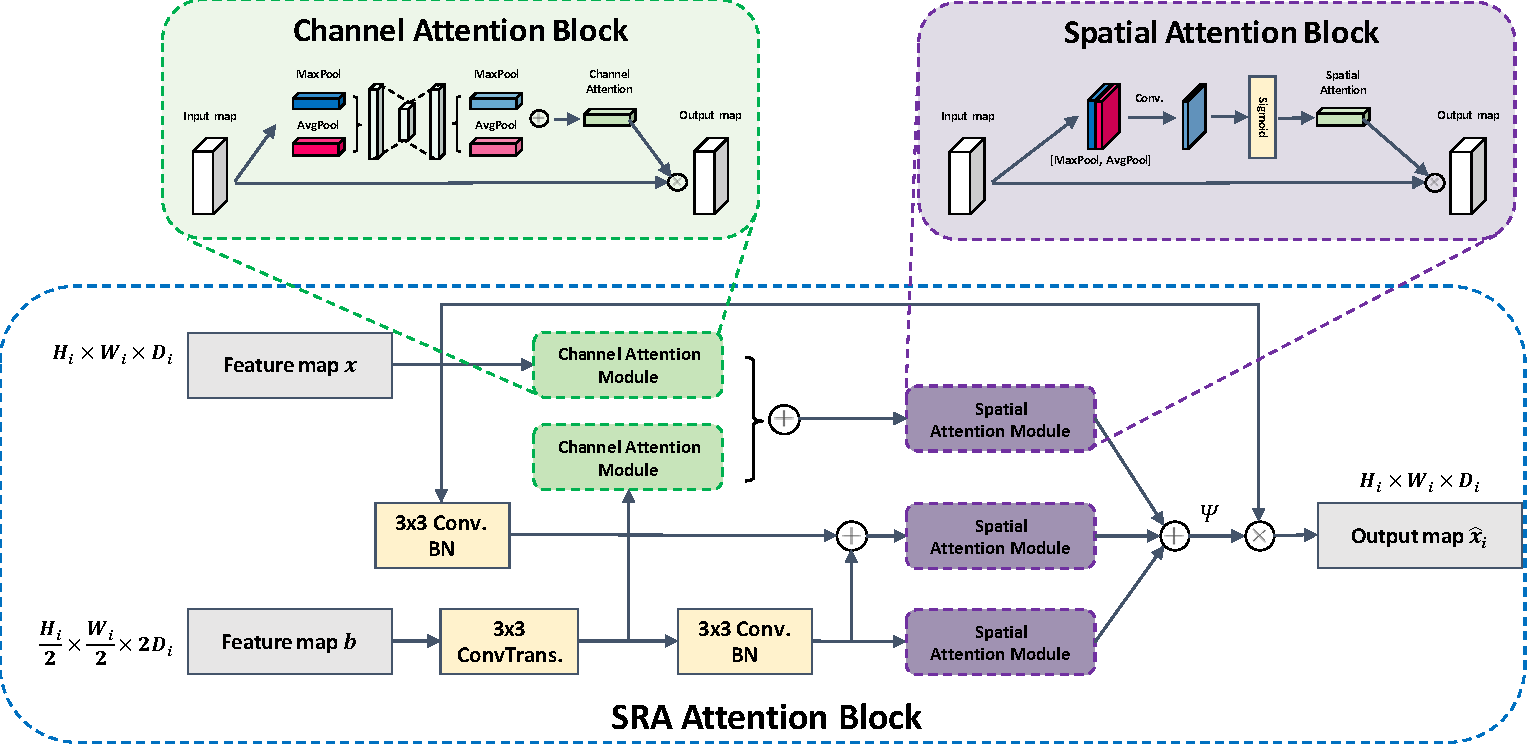
\includegraphics[width=1\textwidth]{figure/Attention.pdf}
  \label{fig:attention}
  \caption{attention}
  \end{figure*}
  
  
  \subsection{Loss function for learning shape}
  \paragraph{Active contour model loss}
  The \emph{Active Contour Models}\cite{Kass1988} are often combined with deep learning models as an attempt to incorporate shape knowledge in the post processing process.
  It converts image segmentation problems into energy minimization problems which goal is optimized towards the object's boundaries.
  Therefore, Chen \emph{et al.} proposed a novel active contour with elastica (ACE) loss function\cite{aceloss} incorporating elastica (curvature and length) and region information as geometrically-natural constraints
  for the image segmentation tasks. The formulation is shown below:
  
  \begin{align}
    Loss_{ACE}=&\underset{Elastica}{\underbrace{\int{\left( \alpha +\beta \times curvature^2 \right)}length}}+\\
    &\lambda \left| \sum_{i=1}^{\Omega}{\sum_{j=1}^{\Omega}{u_{i,j}}\left( c_1-v_{i,j} \right) ^2} \right|+\\
    &\lambda \left| \sum_{i=1}^{\Omega}{\sum_{j=1}^{\Omega}{\left( 1-u_{i,j} \right)}\left( c_2-v_{i,j} \right) ^2} \right|  
  \end{align}
  where the binary ground truth mask and the predicted segmentation are denoted as \(v, u: \Omega \rightarrow \mathbb{R}^{3}\), respectively. 
  $c_1$ and $c_2$ are the mean intensity of the inside (foreground) and outside (background) regions. In our paper, we set $c_{1}=1, c_{2}=0$ empirically.
  \paragraph{BCE loss}
  The binay cross-entropy is the most common use loss function in medical image segmentation tasks, which is defined as:
  \begin{equation}
    L_{BCE}(u, y)=\frac{1}{|\Omega|} \sum_{i}^{\Omega}\sum_{j}^{\Omega}-y_{i,j} \log \left(u_{i,j}\right)-\left(1-y_{i,j}\right) \log \left(1-u_{i,j}\right)
  \end{equation}
  where \(u_{i,j}\) denotes the pixels of the predicted segmentation and \(v_{i,j}\) denotes the pixels of binary ground truth mask.
  
  \paragraph{Dice loss}
  The statistical distributions of labels is easy to makes negative impact on Binary Cross Entropy. 
  Dice loss is another loss function proposed by Milletari\cite{vnet} \emph{et al.}, its purpose is to solve the sample imbalance problem. So we define the Dice loss as the following:
  \begin{align}
    L_{\text {Dice }}(u, y)=1-\frac{2}{K} \sum_{k=0}^{K-1} \frac{\sum_{i}^{\Omega}\sum_{j}^{\Omega} y^{k} u_{i,j}^{k}}{\sum_{i}^{\Omega}\sum_{j}^{\Omega} y_{i,j}^{k}+u_{i,j}^{k}}
  \end{align}
  where \(K\) is the total number of classes, \(u_{i,j}\) denotes the pixels of the predicted segmentation and \(v_{i,j}\) denotes the pixels of binary ground truth mask. In our paper, we set \(K=1\) empirically.
  
  \paragraph{Our proposed}
  为了更好地在训练过程中利用active contour进行学习,并应对正负样本强烈不平衡的场景,我们将 BCE loss, Dice loss and ACE loss 进行结合,并对在训练开始前对\(\alpha, \beta, \theta\)进行预先复制。New loss funciton is formulated below:
  \begin{align}
    loss_{oveall} = \alpha loss_{BCE} + \beta loss_{Dice} + \theta loss_{ACE}
  \end{align}
  
  
  
  
  
  \section{Experiments}
  \subsection{Baseline}
  We used a server equipped with an Intel Core i9-9980XE CPU @ 3.00GHz with 64GB RAM and 12GB of RTX2080Ti GPU for
  our proposed networks training. The operating system of the sever is 64-bits Ubuntu 18.04. The structure of the network 
  is implemented under the open source deep learning library Pytorch with VSCode implementation.
  
  \subsection{Dataset}
  For this study, we conduct our experiments on four differents segmentation tasks. 
  Covering lesions/organs from most commonly used medical imaging modalities including microscopy, 
  computed tomography (CT), and magnetic resonance imaging (MRI).  Table \ref{dataset-table} summarize those datasets in our study.
  
  \begin{table}[htbp]
      \vspace{-2mm}
      \begin{center}\small
      \label{dataset-table}
      \begin{tabular}{ccccc}
        
      \toprule
      Dataset & Image & Input Size & Modality & Provider\\
      \midrule
      Cell & 30 & $512\times 512$  & EM      & ISBI 2012\cite{isbicell}   \\
      Liver    & 4,000 & $512\times 512$       & CT     & LiTS 2017\cite{liver}  \\
      DSB2018      & 670 & $256\times 256$      & EM      & Kaggle\cite{dsb2018} \\
      COVID19         & 1,800 & $630\times 630$     & CT     & Web\cite{covid19,covid19_2}  \\
    \bottomrule    
      \end{tabular}
      \caption{Summaey Of Biomedical Image Segmentation Datasets Used In Our Experiments}
    \end{center}
      %\vspace{-0.35cm}
      \vspace{-4mm}
  \end{table}
    
  
  
  \paragraph{Cell}
  The datset is the segmentation of neuronal structures in electron microscopic recordings.
  The dataset is provided by the EM segmentation challenge\cite{isbicell} that is started at ISBI 2012.
  The data is a set of 30 images ($512\times 512$ pixels) from serial section transmission electron
  microscopy of the Drosophila first instar larva ventral nerve cord (VNC). Each image comes with a corresponding fully annotated ground truth segmentation
  map for cells (white) and membranes (black).
  
  \paragraph{Liver}
  Liver tumor Segmentation Challenge (LiTS)\cite{liver} contain 131 contrast-enhanced CT images provided by hospital around the world with \(512 \times 512\) resolution.
  The ground truth segmentation provides two different labels: liver and lesion. For our experiments,
  we only consider liver as positive class and others as negative class.
  
  
  \paragraph{COVID19}
  Dataset\cite{covid19} includes whole volumes and includes, therefore, both positive and negative slices 
  (373 out of the total of 829 slices have been evaluated by a radiologist as positive and segmented). 
  Dataset\cite{covid19_2} contains 20 CT scans of patients diagnosed with COVID-19 as well as segmentations of lungs and infections made by experts.
  These volumes are converted and normalized in a similar way as above, meanwhile we resize the data to $512\times 512$.
  
  \subsection{Evaluation metrics}
  The experiments are implemented using the Pytorch framework. We use Adam optimizer\cite{Adam} as our
  models' optimizer with a learning rate of 0.00001, batch size of 2. All of datasets are splitted into training set, validation set and test set with 
  the ratio of 8:1:1 using sklearn library. To numerically evaluate, we use five widely adopted metrics, \(i.e.\),
  the Dice similarity coefficient(Dice.), F1 score., Sensitivity(Sen.), Iou. and hausdorff distance(Hd)., the expressions of them are defined as follows:
  \begin{align}
    \text { Sensitivity }=\frac{T P}{T P+F N}
  \end{align}
  \begin{align}
    \operatorname{DSC}(G, S)=\frac{2|G \cap S|}{|G|+|S|}
  \end{align}
  \begin{align}
    \operatorname{IOU}(G, S)=\frac{|G \cap S|}{|G| \cup|S|}
  \end{align}
  \begin{align}
    F_{1}=2 \cdot \frac{\text { precision } \cdot \text { recall }}{\text { precision }+\text { recall }}
  \end{align}
  \begin{align}
    h(G, S)=\max _{g \in G}\left\{\min _{c \in C}\|g-c\|\right\}
  \end{align}
  \subsection{Medical image Segmentation Results}
  For comparsion, we use five origianl network FCN with 32s\cite{fcn}, U-Net\cite{unet}, U-Net++\cite{LiTCLGJW20} , CE-Net\cite{cenet} and U-Net with Attention Gate\cite{attentiongate}
  to evaluate our proposed method. 
  \begin{figure*}[htbp]
    \begin{center}
    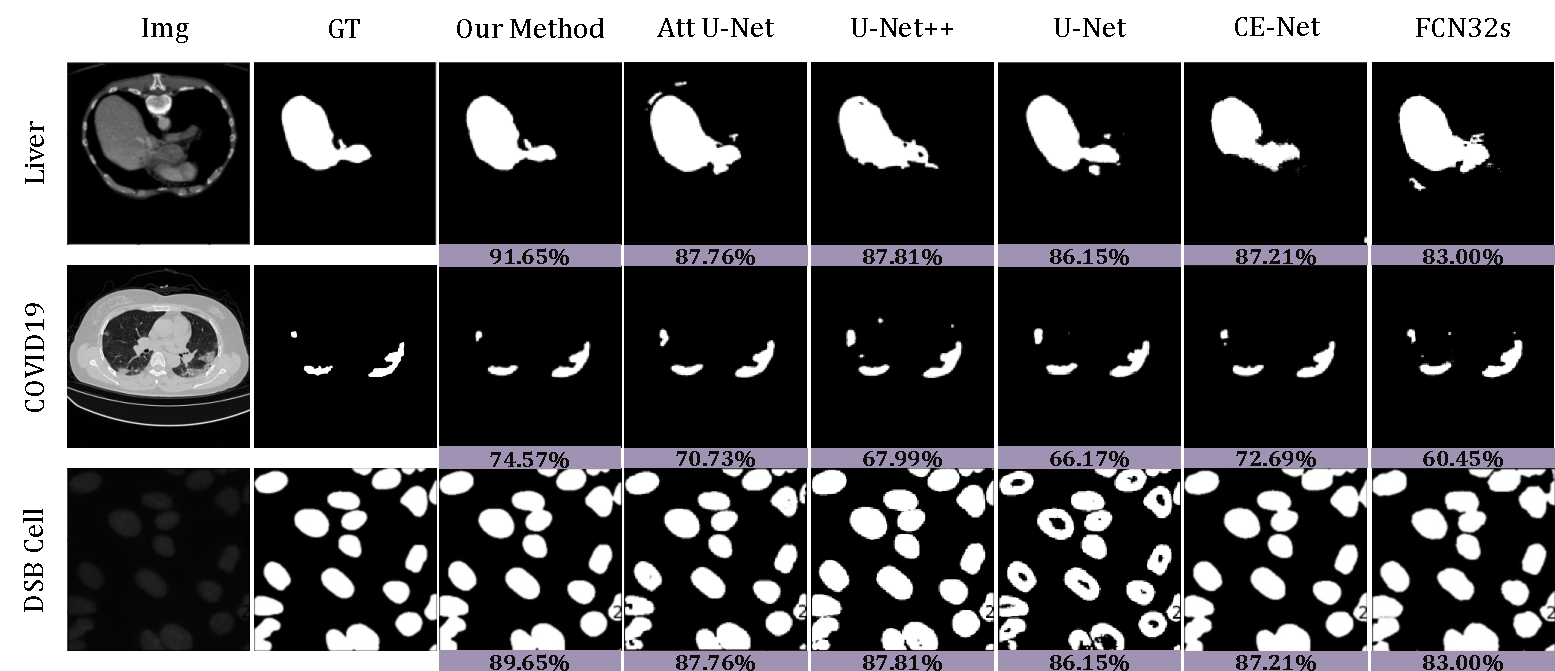
\includegraphics[width=1\textwidth]{figure/result.pdf}
    \vspace{-2mm}
    \caption{Medical image segmentation examples.} 
    \vspace{-2mm}
    \label{fig:result}
    \end{center}
    \vspace{-0.35cm}
  \end{figure*}
  
  We use U-Net and ResU-Net as the baseline to compare with our model on cell, liver and covid19 datasets respectively. In each experiment, the parameters, training set, verification set and test set used are the same.
  
  
  \subsubsection{Live segmentation results}
  Segmentation results of cell segmentation are shown in tables \ref{dataset-table}, 
  
  The experimental results show that the proposed network results in better performance when compared to the state-of-the-art networks(CE-Net, U-Net++, U-Net with Attention Gate, U-Net and FCN32s) by increased 1.30\%, 1.49\%, 4.35\%, 6.11\% and 16.95\% in Dice and F1 score respectively, 
  
  by increased 2.05\%, 2.27\%, 6.08\%, 7.30\% and 19.70\% in Iou index.
  
  by increased 9.80\%, 6.53\%, 7.39\%, 11.81\% and 15.36\% in Sens. index.
  
  by reduced 0.4074, 0.9083, 0.7471, 0.8825 and 2.4968 in Hd. index. 
  
  \begin{table*}[htbp]
  \vspace{-2mm}
  \begin{center}\small
  \label{dataset-table}
  \begin{tabular}{cccccccc}
        
  \toprule
  Datasets & Methods & Shape Loss & Dice. & F1 score. & Iou. & Sens. & Hd.\\
  \midrule
  \multirow{6}{*}{Cell} & Our proposal & $\surd$ & \textbf{0.8588} & \textbf{0.8588} & \textbf{0.7623} & \textbf{0.9296} & \textbf{4.6224}\\
                            & CENet & $\times$ & 0.8458 & 0.8458 & 0.7418 & 0.8316 & 5.2098\\
                            & UNet++ & $\times$ & 0.8439 & 0.8439 & 0.7396 & 0.8643 & 5.5307\\
                            & Attention UNet & $\times$ & 0.8153 & 0.8153 & 0.7015 & 0.8557 & 5.3695\\
                            & UNet  & $\times$  & 0.7977 & 0.7977 & 0.6893 & 0.8115 & 5.5049\\
                            & FCN32s & $\times$ & 0.6895 & 0.6895 & 0.5653 & 0.7760 & 7.1192\\
                            \hline
      \multirow{6}{*}{Liver}   & Our proposal & $\surd$ & \textbf{0.9551} & \textbf{0.9551} & \textbf{0.9165} & \textbf{0.9389} & \textbf{3.8854}\\
                            & U-Net++ & $\times$ & 0.9351 & 0.9351 & 0.8781 & 0.9156 & 5.8218\\
                            & Attention UNet & $\times$ & 0.9346 & 0.9346 & 0.8776 & 0.9056 & 4.836\\
                            & CENet & $\times$ & 0.9315 & 0.9315 & 0.8721 & 0.9045 & 4.904\\
                            & U-Net & $\times$ & 0.9253 & 0.9253 & 0.8615 & 0.9106 & 6.6785\\
                            & FCN32s & $\times$ & 0.9065 & 0.9065 & 0.8300 & 0.9381 & 7.97\\
                            \hline
      \multirow{6}{*}{COVID19} &  Our proposal & $\surd$ & \textbf{0.8489} & \textbf{0.8489} & \textbf{0.7457} & \textbf{0.8570} & \textbf{4.313}\\
                            &  CENet & $\times$ & 0.8348 & 0.8348 & 0.7290 & 0.9359 & 4.7711\\
                            &  UNet++ & $\times$ & 0.8014 & 0.8014 & 0.6799 & 0.9426 & 5.0301\\
                            &  Attention UNet & $\times$ & 0.8229 & 0.8229 & 0.7073 & 0.9435 & 4.8845\\
                            &  UNet  & $\times$ & 0.7874 & 0.7874 & 0.6617 & 0.9528 & 5.2231\\
                            &  FCN32s & $\times$ & 0.7409 & 0.7409 & 0.6045 & 0.9935 & 5.8644\\
    \bottomrule    
      \end{tabular}
      \caption{Comparsion With Other Methods In Cell\cite{dsb2018}, Liver\cite{liver} and COVID19\cite{covid19_2} Dataset}
    \end{center}
      %\vspace{-0.35cm}
  \vspace{-4mm}
  \end{table*}
  \subsubsection{Cell segmentation results}
  
  
  Segmentation results of cell segmentation are shown in table\ref{dataset-table}, 在Dice. and F1 score指数上相比于
  CE-Net, U-Net++, U-Net with Attention Gate, U-Net and FCN32s分别提升了2.01\%, 2.05\%, 2.36\%, 2.98\% and 4.86\%.
  在Iou.指数上,分别提升了3.84\%, 3.89\%, 4.44\%, 5.50\% and 8.65\%. 在Sens.指数上分别提升了2.33\%, 3.33\%, 3.44\%, 
  2.83\% and 0.08\%. 在Hd.指数上分别降低了1.9362, 0.9506, 1.0186, 2.7931 and 4.0846.
  
    \subsubsection{COVID19 segmentation results}
    Segmentation results of covid19 segmentation are shown in table\ref{dataset-table}, 在Dice. and F1 score指数上相比于
    CE-Net, U-Net++, U-Net with Attention Gate, U-Net and FCN32s分别提升了1.41\%, 4.75\%, 2.60\%, 6.15\% and 10.80\%.
    在Iou.指数上,分别提升了1.67\%, 6.58\%, 3.84\%, 8.40\% and 14.12\%. 在Sens.指数上分别提升了2.33\%, 3.33\%, 3.44\%, 2.83\% and 0.08\%.  在Hd.指数上分别降低了0.4581, 0.7171, 0.5715, 0.9101 and 1.5514. 敏感度方面,通过观察Figure 
  \ref{fig:result}我们可以发现,其在分割目标图像时更加保守(改)。
  
  
   综上所述,我们的模型在三个数据集上均consistently outperforms CE-Net and U-Net with Attention-Gate. 
   Figure \ref{fig:result}展示了我们在三个数据集上与其余5个模型的对比示例。COVID-19 ······, Liver ·······, Cell ·······。
  
    \section{Ablation study}
    To justify the effectiveness of the pretrained U-Net\cite{unet}, Res-UNet\cite{ResUNet}, 
    MRC(multi residual convolution) block, RMP block and SAR(spatial channel and gateway) Attention block
    in our proposed method, we conduct the following ablation study using the COVID19 and Cell dataset as examples.
  
    \subsection{Loss function}
    \begin{table*}[htbp]
      \vspace{-2mm}
      \begin{center}\small
          \label{loss-table}
          \begin{tabular}{ccccccc}
              \toprule
              Methods & Loss & Dice. & F1 score. & Iou. & Sens. & Hd.\\
              \midrule
              Our proposal & BCE          & 0.8307 & 0.8307 & 0.7177 & 0.9048 & 4.7641\\
              Our proposal & BCE+DiceLoss & 0.8375 & 0.8375 & 0.7282 & 0.8827 & 4.7241\\
              Our proposal & Ours         & 0.8489 & 0.8489 & 0.7457 & 0.8570 & 4.4313\\
          \bottomrule    
          \end{tabular}
  
  
          \caption{Comparsion With Other loss functions In COVID19\cite{covid19} Dataset}
      \end{center}
      \vspace{-4mm}
    \end{table*}
    为了验证我们使用的损失函数组合模型\(loss_{oveall}\)的有效性,我们以自己设计的模型作为baseline,在其他参数一致的情况下将其与\(loss_{BCE}\)和
    \(loss_{BCE+Dice}\)在COVID19数据集上进行对比,\(loss_{oveall}\)
    和\(loss_{BCE+Dice}\)的定义如下所示:
    \begin{align}
      loss_{oveall} = \alpha loss_{BCE} + \beta loss_{Dice} + \theta loss_{ACE}
    \end{align}
    \begin{align}
      loss_{BCE+Dice} = \alpha loss_{BCE} + \beta loss_{Dice}
    \end{align}
    在本次实验中,我们预先设置\(\alpha=0.5, \beta=0.5\)。对于\(\theta\),因为ACEloss与图像梯度有关,其loss value的范围通常为\([10^1, 10^5]\),所以\(\theta\)值应该
    显著小于\(\alpha, \beta\),在本次试验中,我们预先设置\(\theta=0.0005\)。实验结果如表\ref{loss-table}所示,对比于\(loss_{oveall}\)和\(loss_{BCE+Dice}\),在Dice.指标上
    我们分别提升了4.13\%, 1.14\%; 在F1 score.指标上我们分别提升了4.13\%, 1.14\%; 在Iou.指标上我们分别提升了5.83\%, 1.75\%; 在Sens.指标上我们分别降低了2.02\%, 2.57\%;
    在Hd.指标上我们分别降低了0.5799, 0.2928,其推理结果如图\ref{fig:ablation_loss}所示。
   
    
     
    \begin{figure}[htbp]
      \begin{center}
      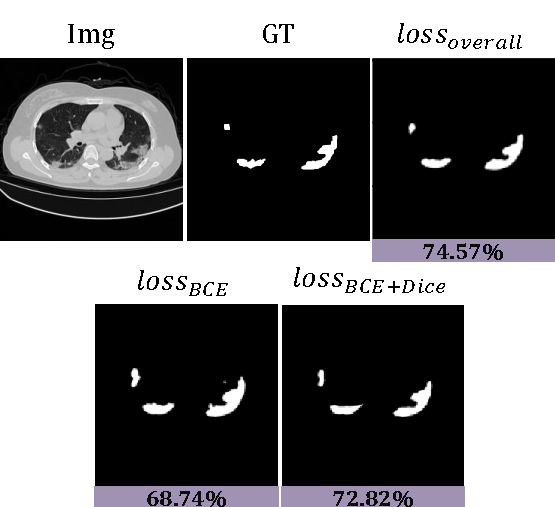
\includegraphics[width=0.45\textwidth]{figure/abliation_loss_img.pdf}
      \vspace{-2mm}
      \caption{不同损失函数训练下的模型推理结果} 
      \vspace{-2mm}
      \label{fig:ablation_loss}
      \end{center}
      \vspace{-0.35cm}
    \end{figure}
  
  
  
  
  \subsection{Modules}
  Our proposed method is based on ResU-Net and our high level feature extractor is based on CE-Net, therefore ResU-Net as well as CE-Net are the most fundamental baseline model.
    To further verify that the modules designed by ourselves are making contribute to segmentation task,
    we combined MRC Block, RMP Block, SRA Attention Block and shape loss function with ResU-Net individually:
    \begin{itemize}
  \item ResU-Net + MRC + RMP: to verify wheather these blocks can ehance the capacity to extract deep image features or not.
  \item ResU-Net + SAR Attention Module: to verify if our Attention module can enhance pixel-wised segmentation from spatial and channels dimensions than skip connection as well as
  attention-gate.
  \item ResU-Net + MRC + RMP +SAR: We use \(loss_{BCE}\) and \(loss_{overall}\) for our model training seperatly, which can enable us to verify the effectiveness of our model。
    \end{itemize}
  
    \begin{table*}[htbp]
      \vspace{-2mm}
      \begin{center}\small
      \label{ablation-table}
      \begin{tabular}{cccccccc}
        
      \toprule
      Dataset & Methods & Loss & Dice. & F1 score. & Iou. & Sens. & Hd.\\
      \midrule
      \multirow{6}{*}{COVID19} & U-Net                & BCE  & 0.7874          & 0.7874          & 0.6617          & 0.9528          & 5.2231        \\
                               & ResU-Net             & BCE  & 0.7988          & 0.7988          & 0.6846          & 0.7969          & 5.1522        \\
                               & ResU-Net + MRC + RMP & BCE  & 0.8185          & 0.8185          & 0.7030          & 0.9295          & 4.8931        \\
                               & ResU-Net + SAR       & BCE  & 0.8105          & 0.8105          & 0.6923          & 0.9601          & 5.0248        \\
                               & ResU-Net+SAR+MRC+RMP & BCE  & 0.8307          & 0.8307          & 0.7177          & 0.9048          & 4.7641        \\
                               & ResU-Net+SAR+MRC+RMP & Ours & \textbf{0.8489} & \textbf{0.8489} & \textbf{0.7457} & \textbf{0.8570} & \textbf{4.313}\\
      \hline
      \multirow{6}{*}{Cell}    & U-Net                & BCE  & 0.7977          & 0.7977          & 0.6893          & 0.8115          & 5.5049\\
                               & ResU-Net             & BCE  & 0.8314          & 0.8314          & 0.7274          & 0.9685          & 5.5861\\
                               & ResU-Net + MRC + RMP & BCE  & 0.8448          & 0.8448          & 0.7414          & 0.9714          & 5.0647\\
                               & ResU-Net + SAR       & BCE  & 0.8545          & 0.8545          & 0.7534          & 0.9669          & 4.9601\\
                               & ResU-Net+SAR+MRC+RMP & BCE  & 0.8525          & 0.8525          & 0.7598          & 0.9744          & 4.9210\\
                               & ResU-Net+SAR+MRC+RMP & Ours & \textbf{0.8588} & \textbf{0.8588} & \textbf{0.7623} & \textbf{0.9296} & \textbf{4.6224}\\
    \bottomrule    
      \end{tabular}
      \caption{Ablation study for each component on COVID19 and Cell dataset}
    \end{center}
      %\vspace{-0.35cm}
      \vspace{-4mm}
    \end{table*}
  
    \paragraph{COVID19 ablation study result}
    我们将上述模型在COVID19数据集上进行测试并对比其IoU, F1 score, Dice, Sensitivity and Hd value. 每次实验所使用的参数,训练集,验证集,测试集均相同。
    如图\ref{fig:covid_comparison}和表\ref{ablation-table}所示:
    ResU-Net with MRC block and RMP block 对比于ResU-Net,Iou.指标提升了1.40\%, F1 score指标提升了1.34\%, Dice指标提升了1.34\%, Sensitivity指标提升了0.29\%, Hd指标降低了0.5214。
    ResU-Net with SRA attention module 对比于ResU-Net,Iou.指标提升了2.60\%, F1 score指标提升了2.31\%, Dice指标提升了2.31\%, Sensitivity指标降低了0.16\%, Hd指标降低了0.6260。
    \begin{figure}[htbp]
      \begin{center}
      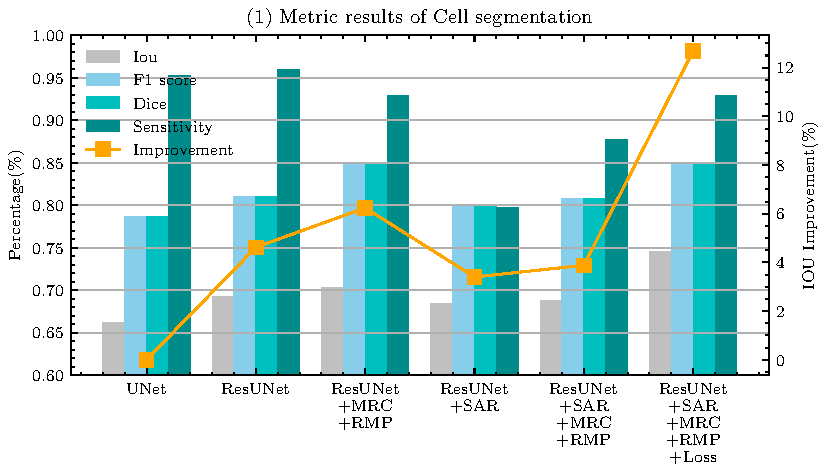
\includegraphics[width=0.45\textwidth]{figure/covid_comparison.pdf}
      \vspace{-2mm}
      \caption{Metric results of COVID19 segmentation compared with different models.} 
      \vspace{-2mm}
      \label{fig:covid_comparison}
      \end{center}
      \vspace{-0.35cm}
    \end{figure}
    ResU-Net with both SRA attention module and MRC, RMP module对比于ResU-Net,Iou.指标提升了3.24\%, F1 score指标提升了2.11\%, Dice指标提升了2.11\%, Sensitivity指标提升了0.59\%, Hd指标降低了0.6651。
    ResU-Net with both SRA attention module and MRC with the combination of shape loss function, 
    Compared RMP module to ResU-Net,Iou.指标提升了3.49\%, F1 score指标提升了2.74\%, Dice指标提升了2.74\%, Sensitivity指标降低了3.89\%, Hd指标降低了0.9637。
    
    \paragraph{Cell ablation study result}
    We further compare our components's performance on Cell dataset.
    我们将上述模型在Cell数据集上进行测试并对比其IoU, F1 score, Dice, Sensitivity and Hd value. 每次实验所使用的参数,训练集,验证集,测试集均相同。
    如图\ref{fig:cell_comparison}和表\ref{ablation-table}所示:
    ResU-Net with MRC block and RMP block 对比于ResU-Net,Iou.指标提升了1.40\%, F1 score指标提升了1.34\%, Dice指标提升了1.34\%, Sensitivity指标提升了0.29\%, Hd指标降低了0.5214。
    ResU-Net with SRA attention module 对比于ResU-Net,Iou.指标提升了2.60\%, F1 score指标提升了2.31\%, Dice指标提升了2.31\%, Sensitivity指标降低了0.16\%, Hd指标降低了0.6260.
    
     
   
      
    \begin{figure}[htbp]
      \begin{center}
      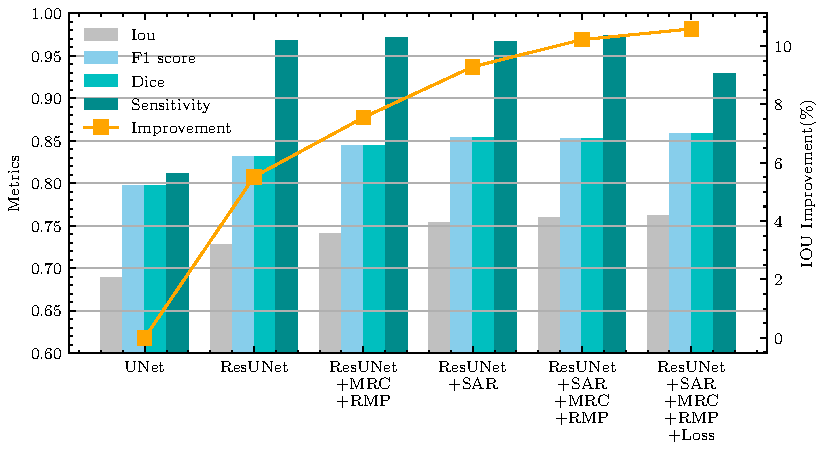
\includegraphics[width=0.45\textwidth]{figure/cell_comparison.pdf}
      \vspace{-2mm}
      \caption{Metric results of Cell segmentation compared with different models.} 
      \vspace{-2mm}
      \label{fig:cell_comparison}
      \end{center}
      \vspace{-0.35cm}
    \end{figure}
    ResU-Net with both SRA attention module and MRC, RMP module对比于ResU-Net,Iou.指标提升了3.24\%, F1 score指标提升了2.11\%, Dice指标提升了2.11\%, Sensitivity指标提升了0.59\%, Hd指标降低了0.6651。
    ResU-Net with both SRA attention module and MRC with the combination of shape loss function, 
    RMP module对比于ResU-Net,Iou.指标提升了3.49\%, F1 score指标提升了2.74\%, Dice指标提升了2.74\%, Sensitivity指标降低了3.89\%, Hd指标降低了0.9637。
    
  Furthermore, 通过将上述模型的IoU指标进行对比,我们可以发现相比于ResU-Net,both MRC+RMP module and SAR attention module 可以有效地提高模型的整体性能,同时两者的结合也能起到不错的提升效果(分别提升了
    1.84\%, 0.64\%)。同时,由于MRC block是CE-Net中DAC block的修改,所以我们也将该模型与CE-Net进行了对比,在IoU识别率仅仅降低了0.04\%的情况下,我们的模型实现了30.17\%的参数精简,提高了训练的速度和节省了模型的显存消耗。
  
  ~\\
  
  \section{Conclusion}\label{sec:conc}
  U-Net is the most prominent deep network in this regard,
  which has been the most popular architecture in the medical imaging community.
  
  Deep learning (DL) based semantic segmentation methods have been providing state-of-the-art performance in the last few years.
  
  

\section{acknowledgment}

\bibliographystyle{IEEEtran}
\bibliography{complete.bib}

\begin{IEEEbiography}[{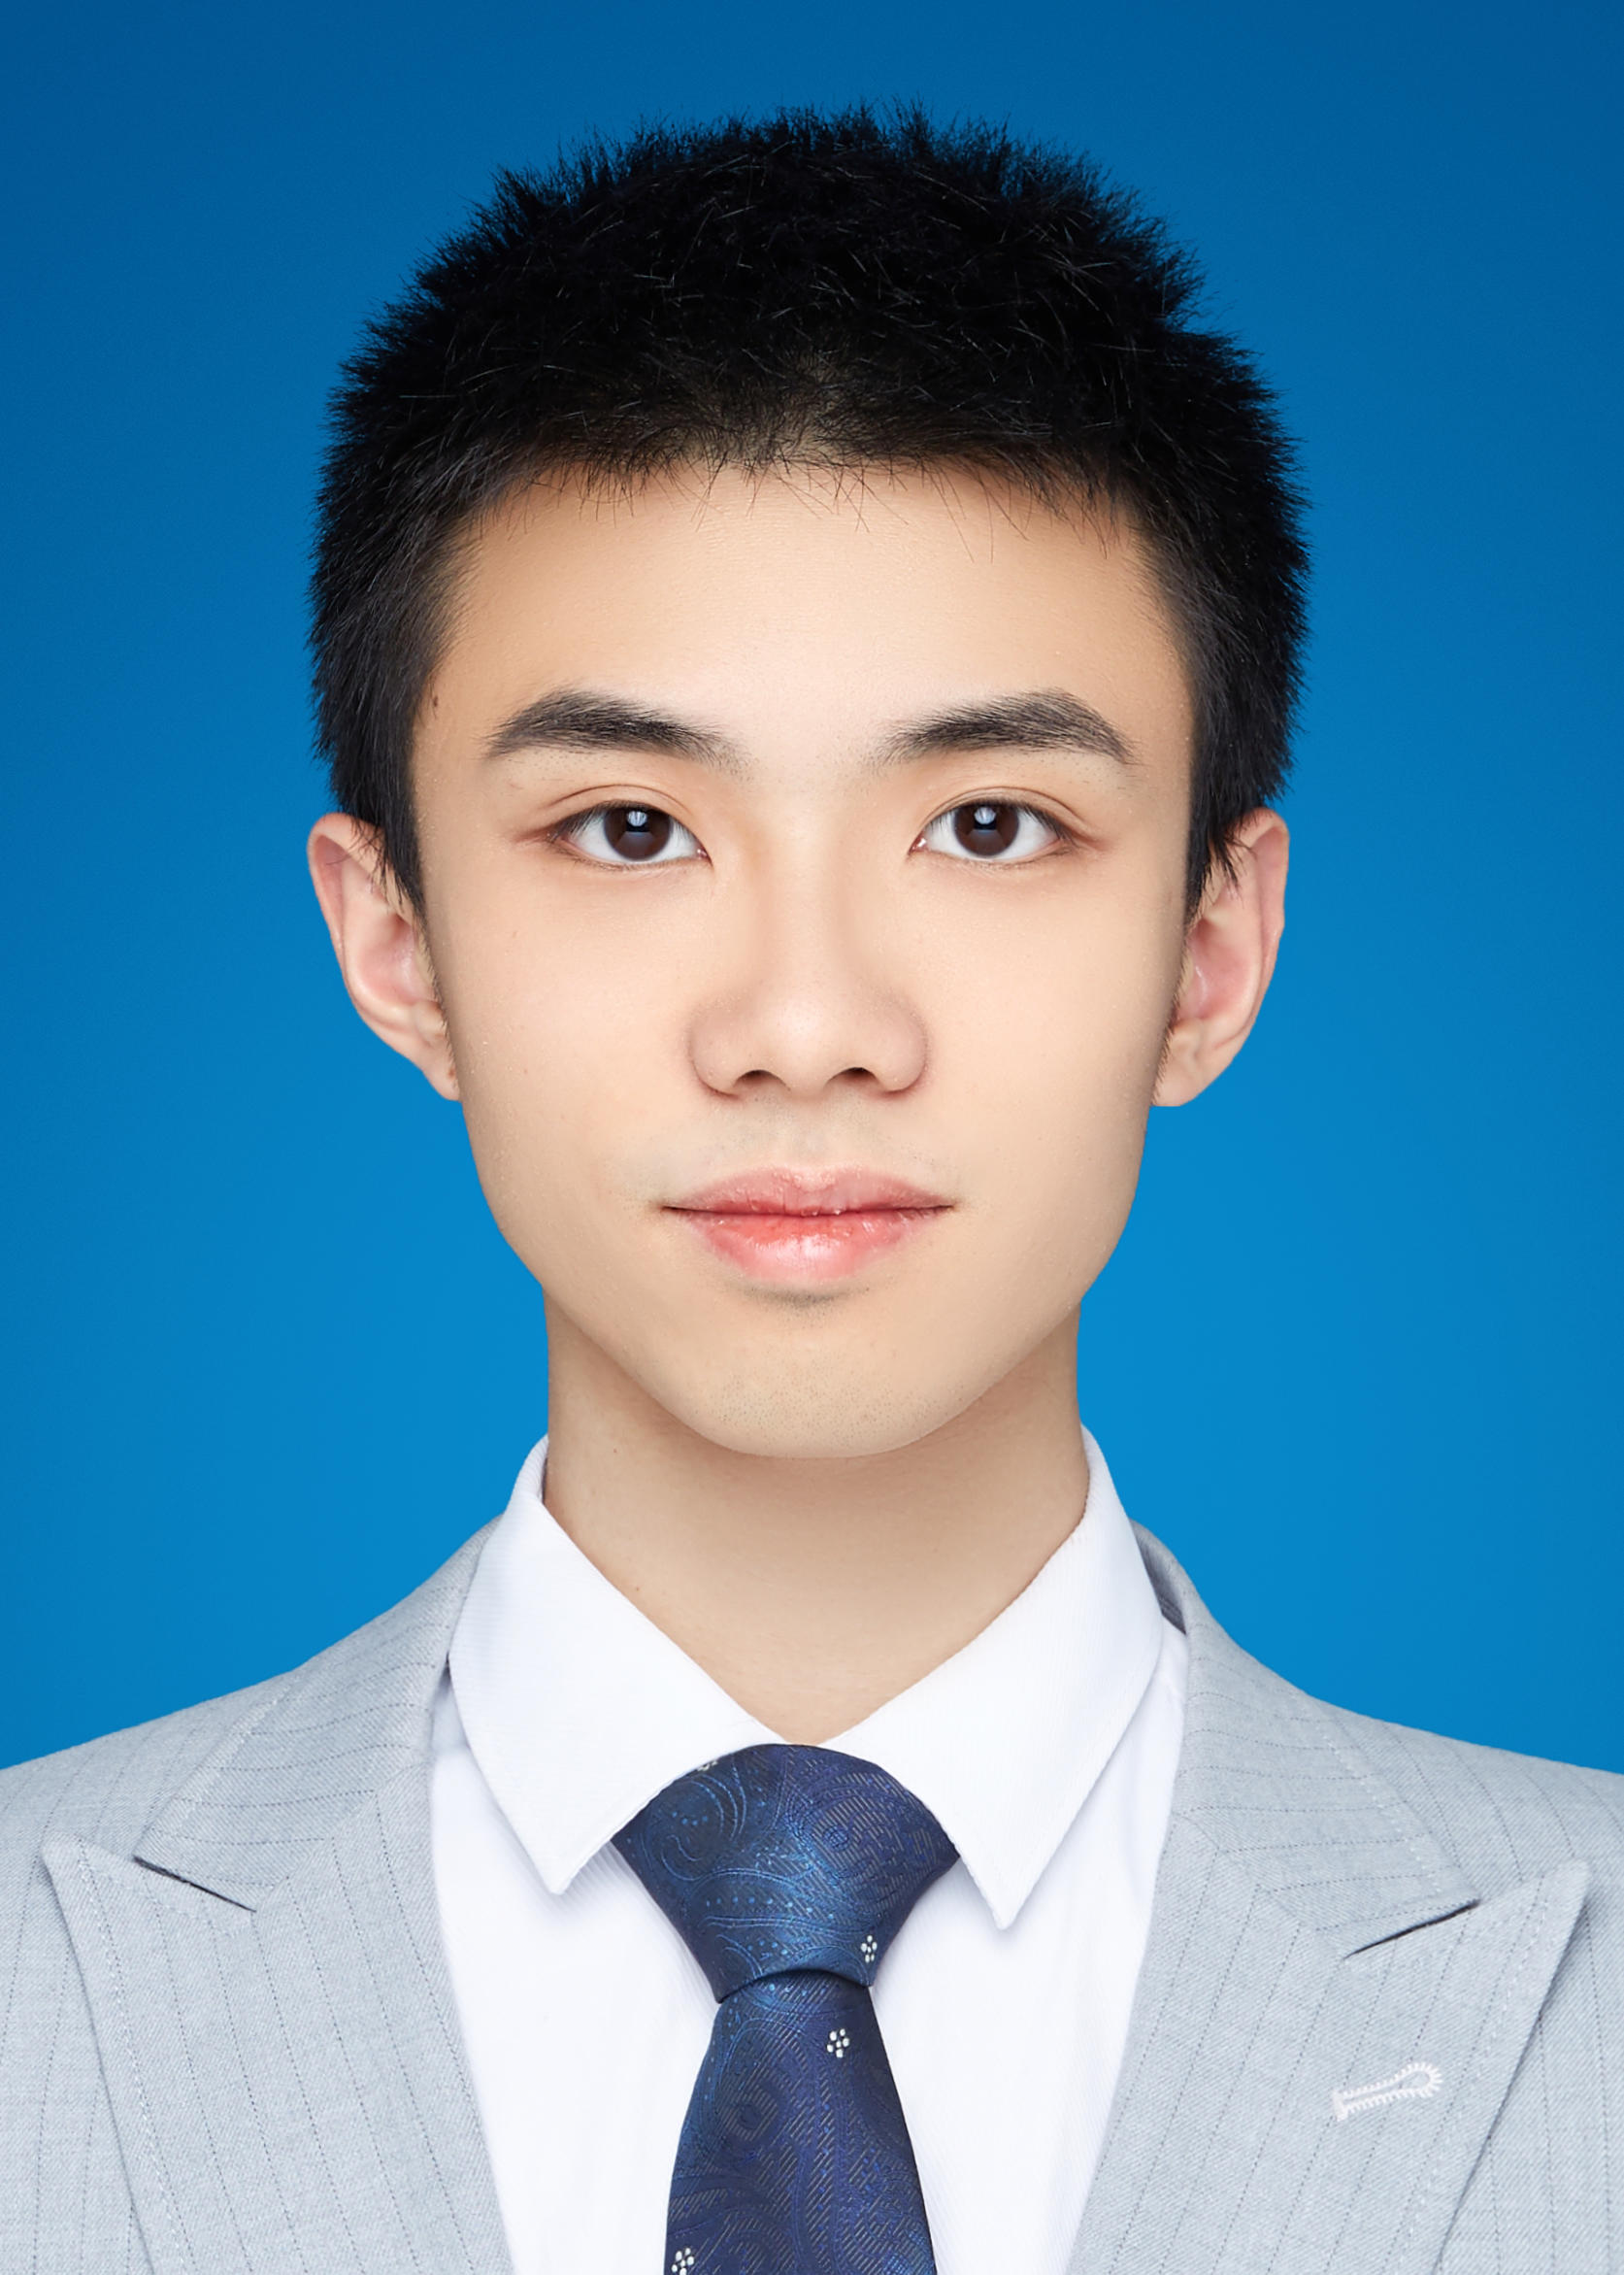
\includegraphics[width=1in,height=1.25in,clip,keepaspectratio]{lihao.png}}]{HAO LI} 
  is currently pursuing his bachelor's with the College of Information Science and Technology, Beijing University of Chemical Technology, Beijing.

  His research interest include robotics, computer vision and deep learning.
\end{IEEEbiography}

\begin{IEEEbiography}[{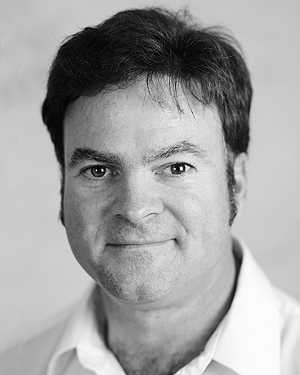
\includegraphics[width=1in,height=1.25in,clip,keepaspectratio]{a2.png}}]{Second B. Author} was born in Greenwich Village, New York, NY, USA in 
1977. He received the B.S. and M.S. degrees in aerospace engineering from 
the University of Virginia, Charlottesville, in 2001 and the Ph.D. degree in 
mechanical engineering from Drexel University, Philadelphia, PA, in 2008.

From 2001 to 2004, he was a Research Assistant with the Princeton Plasma 
Physics Laboratory. Since 2009, he has been an Assistant Professor with the 
Mechanical Engineering Department, Texas A{\&}M University, College Station. 
He is the author of three books, more than 150 articles, and more than 70 
inventions. His research interests include high-pressure and high-density 
nonthermal plasma discharge processes and applications, microscale plasma 
discharges, discharges in liquids, spectroscopic diagnostics, plasma 
propulsion, and innovation plasma applications. He is an Associate Editor of 
the journal \emph{Earth, Moon, Planets}, and holds two patents. 

Dr. Author was a recipient of the International Association of Geomagnetism 
and Aeronomy Young Scientist Award for Excellence in 2008, and the IEEE 
Electromagnetic Compatibility Society Best Symposium Paper Award in 2011. 
\end{IEEEbiography}


\EOD

\end{document}
